\subsection{Co-Design Problems\label{sec:Design-Problems}}

The basic objects considered in this paper are ``design problems'',
of which several classes will be investigated. We start by defining
a ``design problem with implementation'', which is a tuple of ``\F{functionality}
space'', ``\Icol{implementation} space'', and ``\R{resources}
space'', together with two maps that describe the feasibility relations
between these three spaces~(\cref{fig:setup}).
\begin{definition}
\label{def:design_problem}A \emph{design problem with implementation}
(DPI) is a tuple
\begin{equation*}
  \tup{\F{F},\R{R},\Icol{I},\exc,\eval}  
\end{equation*}
where:

\begin{itemize}
\item $\funsp$ is a poset, called \emph{\F{functionality} space};
\item $\ressp$ is a poset, called \emph{\R{resources} space};
\item $\impsp$ is a set, called \emph{\Icol{implementation} space};
\item the map~$\exc\colon\impsp\rightarrow\funsp$, mnemonics for ``execution'',
maps an implementation to the functionality it provides;
\item the map~$\eval\colon\impsp\rightarrow\ressp$, mnemonics for ``evaluation'',
maps an implementation to the resources it requires.
\end{itemize}

\begin{figure}[h]
\begin{center}
    \includegraphics[scale=0.33]{gmcdp_setup}
\end{center}
\caption{\label{fig:setup}}
\end{figure}
\todo{Redo figure with consistent style}
\end{definition}


A graphical notation will help reasoning about composition. A DPI is represented as a box with~$\dpinumf$ green edges and~$\dpinumr$ red edges~(\cref{fig:dp_graphical}).

\begin{figure}[h]
    \centering
    \includegraphics[scale=0.5]{gmcdp_dp_graphical.pdf}
    \caption{\label{fig:dp_graphical}}
\end{figure}
\todo{Redo figure with consistent style}
%\captionsideleft{\label{fig:dp_graphical}}{\includegraphics[scale=0.33]{gmcdp_dp_graphical.pdf}}

\noindent This means that the functionality and resources spaces
can be factorized in~$\dpinumf$ and~$\dpinumr$ components: $\funsp=\prod_{i=1}^{\dpinumf}\pi_{i}\funsp_{i},$
$\ressp=\prod_{j=1}^{\dpinumr}\pi_{j}\ressp$, where ``$\pi_{i}$''
represents the projection to the $i$-th component. If there are no
green (respectively, red) edges, then $\dpinumf$ (respectively, $\dpinumr$)
is zero, and $\funsp$ (respectively, $\ressp$) is equal to~$\One=\{\left\langle \right\rangle \}$,
the set containing one element, the empty tuple~$\left\langle \right\rangle $.

These \emph{co-design diagrams} are not to be confused with signal
flow diagrams, in which the boxes represent oriented systems and the
edges represent signals.


\begin{example}[Motor design]
\label{exa:motor}Suppose we need to choose a motor for a robot from
a given set. The \emph{functionality} of a motor could be parametrized
by \F{torque} and \F{speed}. The \emph{resources} to consider
could include the \R{cost {[}\${]}}, the \R{mass {[}g{]}}, the
input \R{voltage {[}V{]}}, and the input \R{current {[}A{]}}.
The map~$\exc:\impsp\rightarrow\funsp$ assigns to each motor its
functionality, and the map~$\eval:\impsp\rightarrow\ressp$ assigns
to each motor the resources it needs~(\cref{fig:motor}).
\end{example}

\begin{figure}[h]
    \centering
\includegraphics[scale=0.5]{gmcdp_motor_evalexec}
    \caption{\label{fig:motor_evalexec}}
\end{figure}
\todo{Redo figure with consistent style}
%\captionsideleft{\label{fig:motor_evalexec}}{\includegraphics[scale=0.33]{gmcdp_motor_evalexec}}


\begin{example}[Chassis design]
\label{exa:chassis}Suppose we need to choose a chassis for a robot~(\cref{fig:gmcdp_chassis_eval}).
The implementation space~$\impsp$ could be the set of all chassis
that could ever be designed (in case of a theoretical analysis), or
just the set of chassis available in the catalogue at hand (in case
of a practical design decision). The functionality of a chassis could
be formalized as ``the ability to transport a certain \F{payload
{[}g{]}}'' and ``at a given \F{speed {[}m/s{]}}''. More refined
functional requirements would include maneuverability, the cargo volume,
etc. The resources to consider could be the \R{cost {[}\${]}} of
the chassis; the total mass; and, for each motor to be placed in the
chassis, the required \R{speed {[}rad/s{]}} and \R{torque {[}Nm{]}}.
\end{example}
\begin{figure}[h]
    \centering
    \includegraphics[scale=0.5]{gmcdp_chassis_eval.pdf}
    \caption{\label{fig:gmcdp_chassis_eval}}
\end{figure}
\todo{Redo figure with consistent style}
%\captionsideleft{\label{fig:gmcdp_chassis_eval}}{\includegraphics[scale=0.33]{gmcdp_chassis_eval.pdf}}
 

\subsubsection{Mechatronics}


Many mechanisms can be readily modeled as relations between a provided
functionality and required resources.


\begin{example}
The \F{functionality} of a DC motor~(\figref{dc_motor})
is to provide a certain \F{speed} and \F{torque}, and the \R{resources}
are \R{current} and \R{voltage}.
\end{example}

\begin{figure}[h]
    \centering
    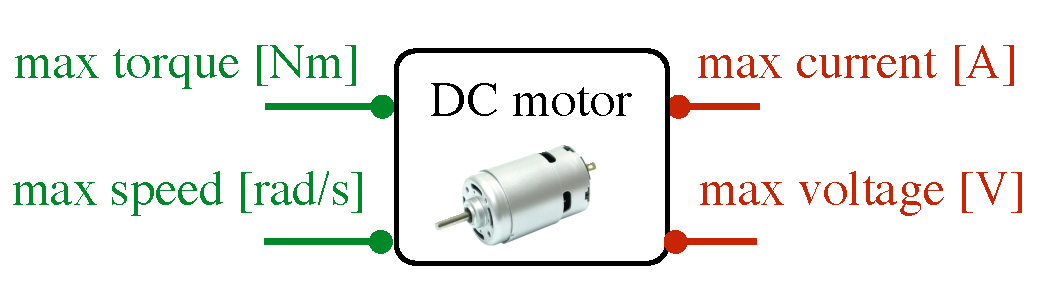
\includegraphics[scale=0.33]{reits2_DC_motor.pdf}
\caption{\label{fig:dc_motor}}
\end{figure}


\begin{figure}[h]
    \centering
    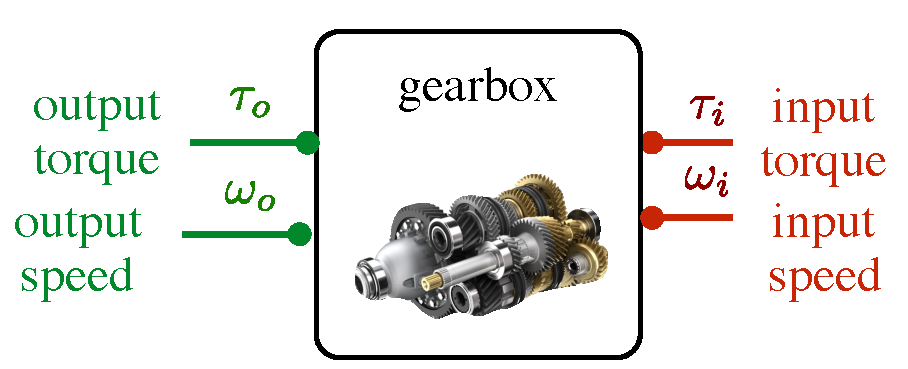
\includegraphics[scale=0.33]{reits2_gearbox}
    \caption{ \label{fig:gearbox}}
\end{figure}

\begin{example}
A gearbox (\figref{gearbox}) provides a certain \F{output
torque $\tau_o$} and \F{speed $\tau_o$}, given a certain
\R{input torque $\tau_i$} and \R{speed $\omega_i$}. For
an ideal gearbox with a reduction ratio $r \in \mathbb{ℚ}_+$ and
efficiency ratio $\gamma$, $0<\gamma<1$, the constraints among
those quantities are ${\colR \omega_i}\geq r\,{\colF \omega_o}$
and ${\colR \tau_i\omega_i}\geq\gamma\,{\colF \tau_o\omega_o}.$
\end{example}


\begin{example}
\emph{Propellers}~(\figref{propeller}) generate \F{thrust}
given a certain \R{torque} and \R{speed}.
\end{example}

\begin{figure}[h!]
    \centering
    \includegraphics[scale=0.33]{reits2_propellers}
\caption{} \label{fig:propeller}
\end{figure}

\begin{example}
A \emph{crank-rocker} (\figref{crack}) converts \R{rotational
motion} into a \F{rocking motion}.
\end{example}

\begin{figure}[h!] 
    \centering
    \includegraphics[scale=0.33]{reits2_crank_rocker}
    \caption{
        \label{fig:crack}}
    \end{figure}

\subsubsection{Geometrical constraints}

Geometrical constraints are examples of constraints that are easily
recognized as monotone, but possibly hard to write down in closed
form.

\begin{example}[Bin packing]
Suppose that each internal component occupies a volume
bounded by a parallelepiped, and that we must choose the minimal enclosure
in which to place all components~(\figref{packing}). What
is the minimal size of the enclosure? This is a variation of the \emph{bin
packing} problem, which is in NP for both 2D and 3D~\cite{lodi02two}.
It is easy to see that the problem is monotone, by noticing that,
if one the components shapes increases, then the size of the enclosure
cannot shrink.
\end{example}

\begin{figure}[h]
    \centering

\includegraphics[scale=0.33]{reits2_fit_boxes}
\caption{\label{fig:packing}}
\end{figure}


\subsubsection{Inference}

Many inference problems have a monotone formalization, taking the
\F{accuracy} or \F{robustness} as functionality, and \R{computation}
or \R{sensing} as resources. Typically these bounds are known in
a closed form only for restricted classes of systems, such as the
linear/Gaussian setting.

\begin{example}
(SLAM) One issue with particle-filter-based estimation procedures,
such as the ones used in the popular GMapping~\cite{grisetti07improved}
method, is that the filter might diverge if there aren't enough particles.
Although the relation might be hard to characterize, there is a monotone
relation between the \F{robustness} (1 - probability of failure),
the \F{accuracy}, and the \R{number of particles}~(\figref{gmapping}).
\end{example}

\begin{figure}[h]
    \centering
\includegraphics[scale=0.33]{reits2_particlefilter}
\caption{\label{fig:gmapping} }
\end{figure}



\begin{example}
(Stereo reconstruction) Progressive reconstruction system (e.g.,~\cite{locher16progressive}),
which start with a coarse approximation of the solution that is progressively
refined, are described by a smooth relation between the \F{resolution}
and the \R{latency} to obtain the answer~(\figref{progressive}).
A similar relation characterizes any anytime algorithms in other domains,
such as robot motion planning.
\end{example}

\begin{figure}[h]
    \centering
    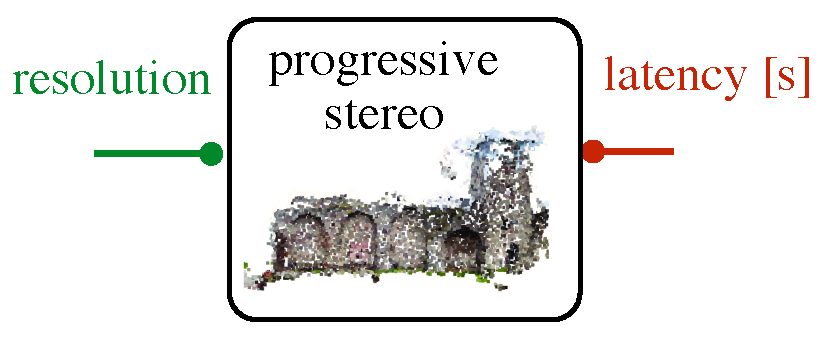
\includegraphics[scale=0.33]{reits2_progressive_stereo}
    \caption{\label{fig:progressive}}
\end{figure}

\begin{example}
The empirical characterization of the monotone relation between \F{the
accuracy of a visual SLAM solution} and \R{the power consumption}
is the goal of recent work by Davison and colleagues~\cite{nardi15introducing,zia16comparative}.
\end{example}


\subsubsection{Communication}

\begin{example}[Transducers]
Any type of "transducer" that bridges between different
mediums can be modeled as a DP. For example, an access point~(\figref{accesspoint})
provides the \F{"wireless access"} functionality, and requires
that the infrastructure provides the \R{"Ethernet access"} resource.
\end{example}

\begin{figure}[h] 
    \centering
    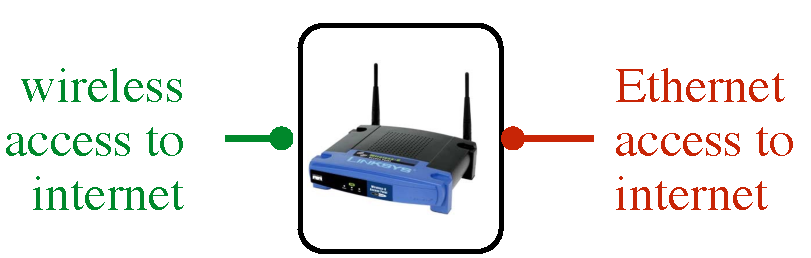
\includegraphics[scale=0.33]{reits2_network2}
    \caption{\label{fig:accesspoint}}

\end{figure}


\newcommand{\Rcpu}[1]{\mathbb{R}^{\!\!\!\!\!\textrm{[#1]}}}

\begin{example}[Wireless link]
The basic functionality of a wireless link is to provide
a certain \F{bandwidth}. Further refinements could include bounds
on the latency or the probability that a packet drop is dropped. Given
the established convention about the the preference relations for
functionality, in which a \emph{lower} functionality is "easier"
to achieve, one needs to choose "\F{\emph{minus} the latency}"
and "\F{\emph{minus} the packet drop probability}" for them
to count as functionality. As for the resources, apart from the \R{transmission
power [W]}, one should consider at least \R{the spectrum occupation},
which could be described as an interval $[f_0,f_1]$ of the frequency
axis $\Rcpu{Hz}$. Thus the resources space is $ℛ=\colR\Rcpu{W}×\vmath{intervals}(\Rcpu{Hz})$.
\end{example}

\begin{figure}[h]
    \centering
    \includegraphics[scale=0.33]{reits2_communication}
    \caption{ \label{fig:networklink}}
    \end{figure}


\subsubsection{Multi-robot systems}

In a multi-robot system there is always a trade-off between the number
of robots and the capabilities of the single robot.
\begin{example}
Suppose we need to create a swarm of agents whose functionality is
\F{to sweep an area}. If the functionality is fixed, one expects
a three-way trade-off between the three resources: number of agents,
the speed of a single agent, and the execution time. For example,
if the time available decreases, one has to increase either the speed
of an agent or the number of agents~(\figref{multirobot2}).
\end{example}

\begin{figure}[h]
\subfloat[]{
\includegraphics[scale=0.33]{reits2_multirobot}

}\subfloat[\label{fig:multirobot2}]{
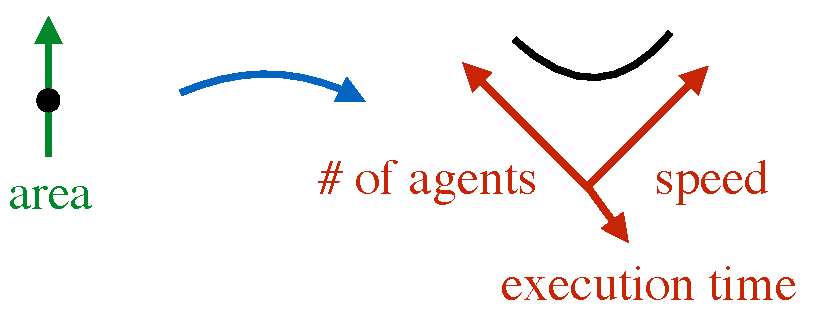
\includegraphics[scale=0.33]{reits2_multirobot2}

}\caption{}
\end{figure}
 

\subsubsection{LQG Control}

\todo[inline]{Write short summary}



\subsubsection{Computation}

% keep wrapped
\begin{wrapfigure}{r}{0\columnwidth}
\includegraphics[scale=0.33]{reits2_cpu_simple}\caption{}
\end{wrapfigure}
\leavevmode

The trivial model of a CPU is as a device that provides \F{computation,
measured in flops}, and requires \R{power [W]}. Clearly there
is a monotone relation between the two.

A similar monotone relation between application requirements and computation
resources holds in a much more general setting, where both application
and computation resources are represented by graphs. This will be
an example of a monotone relation between nontrivial partial orders.

In the Static Data Flow (SDF) model of computation~\cite[Chapter 3]{sriram00,lee10},
the application is represented as a graph of procedures that need
to be allocated on a network of processors.

% keep wrapped
\begin{wrapfigure}{r}{0\columnwidth}
\includegraphics[scale=0.33]{reits2_small_app_graph}
\end{wrapfigure}

Define the\emph{ application graph }(sometimes called "computation
graph") as a graph where each node is a procedure (or "actor")
and each edge is a message that needs to be passed between procedures.
Each node is labeled by the number of ops necessary to run the procedure.
Each edge is labeled by the size of the message. There is a partial
order $ \leq$ on application graphs. In this order, it holds that $A_1 \leq A_2$
if the application graph $A_2$ needs more computation or bandwidth
for its execution than $A_1$. Formally, it holds that $A_1 \leq A_2$
if there is a homomorphism $\varphi:A_1  \Rightarrow A_2$; and,
for each node $n∈A_1$, the node $\varphi(n)$ has equal or
larger computational requirements than $n$; and for each edge $⟨n_1,n_2⟩ $
in $A_2$, the edge $⟨\varphi(n_1),\varphi(n_2)⟩ $
has equal or larger message size.

\begin{wrapfigure}{r}{0\columnwidth}
\includegraphics[scale=0.33]{reits2_small_res_graph}\end{wrapfigure}

Define a\emph{ resource graph} as a graph where each node represents
a processor, and each edge represents a network link. Each node is
labeled by the processor capacity [flops] Each edge is labeled
by latency [s] and bandwidth [B/s]. There is a partial order
on resources graph as well: it holds that $R_1 \leq R_2$ if
the resource graph $R_2$ has more computation or network available
than $R_1$. The definition is similar to the case of the application
graph: there must exist a graph homomorphism $\varphi:R_1  \Rightarrow R_2$
and the corresponding nodes (edges) of $R_2$ must have larger
or equal computation (bandwidth) than those of $R_1$.

\begin{wrapfigure}{r}{0\columnwidth}
\includegraphics[scale=0.33]{reits2_small_allocation}\end{wrapfigure}

Given an application graph $A$ and a resource graph $R$, a typical
resource allocation problem consists in choosing in which processor
each actor must be scheduled to maximize the throughput $T$~[Hz].
This is equivalent to the problem of finding a graph homomorphism $\Psi:A \Rightarrow R$.
Let $T^{\ast}$ be the optimal throughput, and write it as a function
of the two graphs:
\[
T^{\ast}=T^{\ast}(A,R).
\]
Then the optimal throughput $T^{*}$ is decreasing in $A$ (a more
computationally demanding application graph decreases the throughput)
and increasing in $R$ (more available computation/bandwidth increase
the throughput).

Therefore, we can formalize this as a design problem where the two
functionalities are \F{the throughput $T$ [Hz]} and \F{the
application graph $A$}, and the \R{resource graph $R$} is the
resource.

\begin{figure}

\includegraphics[scale=0.33]{reits2_resourcegraph1}

\caption{}
\end{figure}



\begin{example}
Svorenova\,\,\etal~\cite{svorenova16resource} consider a joint
sensor scheduling and control synthesis problem, in which a robot
can decide to not perform sensing to save power, given performance
objectives on the probability of reaching the target and the probability
of collision. The method outputs a Pareto frontier of all possible
operating points. This can be cast as a design problem with functionality
equal to the \F{probability of reaching the target} and (the inverse
of) \F{the collision probability}, and with resources equal to the
\R{actuation power}, \R{sensing power}, and \R{sensor accuracy}.
    
\end{example}
\captionsideleft{\label{fig:progressive-1-1}}{\includegraphics[scale=0.33]{batteries_svorenova.pdf}}


\begin{example}
Nardi\,\,\etal~\cite{zia16comparative} describe a benchmarking
system for visual SLAM that provides the empirical characterization
of the monotone relation between \F{the accuracy} of the visual
SLAM solution, the \F{throughput {[}frames/s{]}} and \R{the energy
for computation {[}J/frame{]}}. The implementation space is the product
of algorithmic parameters, compiler flags, and architecture choices,
such as the number of GPU cores active. This is an example of a design
problem whose functionality-resources map needs to be experimentally
evaluated.
\end{example}
\captionsideleft{}{\includegraphics[scale=0.33]{batteries_zia.pdf}}

\subsubsection{Other examples in minimal robotics}

Many works have sought to find ``minimal'' designs for robots, and
can be understood as characterizing the relation between the poset
of \F{tasks} and the poset of physical resources, which is the product
of \R{sensing}, \R{actuation}, and \R{computation} resources,
plus other non-physical resources, such as \R{prior knowledge}~(\cref{fig:robot-generic}).
Given a task, there is a minimal antichain in the resources poset
that describes the possible trade-offs (e.g., compensating lousier
sensors with more computation). 

\captionsideleft{\label{fig:robot-generic}}{\includegraphics[scale=0.33]{batteries_okane.pdf}}

The poset structure arises naturally: for example, in the \emph{sensor
lattice}~\cite{lavalle12sensing}\emph{,} a sensor dominates another
if it induces a finer partition of the state space. Similar dominance
relations can be defined for actuation and computation. O'Kane and
Lavalle~\cite{okane08comparing} define a robot as a union of ``robotic
primitives'', where each primitive is an abstraction for a set of
sensors, actuators, and control strategies that can be used together
(e.g., a compass plus a contact sensor allow to ``drive North until
a wall is hit''). The effect of each primitive is modeled as an operator
on the robot's information space. It is possible to work out what
are the minimal combinations of robotic primitives (minimal antichain)
that are sufficient to perform a task (e.g., global localization),
and describe a dominance relation (partial order) of primitives. Other
works have focused on minimizing the complexity of the controller.
Egerstedt~\cite{egerstedt03motion} studies the relation between
the \F{complexity of the environment} and a notion of \R{minimum
description length of control strategies}, which can be taken as
a proxy for the computation necessary to perform the task. Soatto~\cite{soatto11steps}
studies the relation between the \F{performance of a visual task},
and the \R{ minimal representation} that is needed to perform that
task. 





\subsection{Co-design problems\label{sec:Co-design-problems}}

A ``co-design problem'' will be defined as a multigraph of design
problems. Graphically, one is allowed to connect only edges of different
color. This interconnection is indicated with the symbol~``$\posleq$''
in a rounded box~(\cref{fig:connection}). 

\captionsideleft{\label{fig:connection}}{\includegraphics[scale=0.33]{papers/uncertainty/unc_connection.pdf}}

\noindent The semantics of the interconnection is that the resources
required by the first DPI are provided by the second DPI. This is
a partial order inequality constraint of the type~$\res_{1}\posleq\funn_{2}$.

\begin{definition}
\label{def:cdpi}A \emph{Co-Design Problem with Implementation} (CDPI)
is a tuple $\left\langle \funsp,\ressp,\left\langle \cdpiN,\mathcal{E}\right\rangle \right\rangle ,$
where~$\funsp$ and~$\ressp$ are two posets, and~$\left\langle \cdpiN,\mathcal{E}\right\rangle $
is a\emph{ }multigraph of DPIs. Each node~$\cdpin\in\cdpiN$ is a
DPI $\cdpin=\left\langle \funsp_{\cdpin},\ressp_{\cdpin},\impsp_{\cdpin},\exc_{\cdpin},\eval_{\cdpin}\right\rangle .$
An edge~$e\in\mathcal{E}$ is a tuple $e=\left\langle \left\langle \cdpinA,\cdpiresindA\right\rangle ,\left\langle \cdpinB,\cdpifunindB\right\rangle \right\rangle $,
where~$\cdpinA,\cdpinB\in\cdpiN$ are two nodes and~$\cdpiresindA$
and~$\cdpifunindB$ are the indices of the components of the functionality
and resources to be connected, and it holds that~$\pi_{\cdpiresindA}\ressp_{\cdpinA}=\pi_{\cdpifunindB}\funsp_{\cdpinB}$~(\cref{fig:mcdps}). 

\captionsideleft{\label{fig:mcdps}}{\includegraphics[scale=0.33]{gmcdptro_cdpi.pdf}}
\end{definition}

A CDPI is equivalent to a DPI with an implementation space~$\impsp$
that is a subset of the product $\prod_{\cdpin\in\cdpiN}\impsp_{\cdpin}$,
and contains only the tuples that satisfy the co-design constraints.
An implementation tuple~$\imp\in\prod_{\cdpin\in\cdpiN}\impsp_{\cdpin}$
belongs to~$\impsp$ iff it respects all functionality\textendash resources
constraints on the edges, in the sense that, for all edges~$\left\langle \left\langle \cdpinA,\cdpiresindA\right\rangle ,\left\langle \cdpinB,\cdpifunindB\right\rangle \right\rangle $
in~$\mathcal{E}$, it holds that 
\[
\pi_{\cdpiresindA}\eval_{\cdpinA}(\pi_{\cdpinA}\imp)\posleq\pi_{\cdpifunindB}\exc_{\cdpinB}(\pi_{\cdpinB}\imp).
\]
The posets~$\funsp,\ressp$ for the entire CDPI are the products
of the functionality and resources of the nodes that remain unconnected.
For a node~$\cdpin$, let~$\unconnectedfun_{\cdpin}$ and~$\unconnectedres_{\cdpin}$
be the set of unconnected functionalities and resources. Then~$\funsp$
and~$\ressp$ for the CDPI are defined as the product of the unconnected
functionality and resources of all DPIs: $\funsp=\prod_{\cdpin\in\cdpiN}\prod_{\cdpifunind\in\unconnectedfun_{\cdpin}}\pi_{\cdpifunind}\funsp_{\cdpin}$
and $\ressp=\prod_{\cdpin\in\cdpiN}\prod_{\cdpiresind\in\unconnectedres_{\cdpin}}\pi_{\cdpiresind}\ressp_{\cdpin}.$
The maps $\exc,\eval$ return the values of the unconnected functionality
and resources:
\begin{align*}
\exc:\imp & \mapsto{\scriptstyle {\displaystyle \prod_{\cdpin\in\cdpiN}\prod_{\cdpifunind\in\unconnectedfun_{\cdpin}}}}\pi_{\cdpifunind}\exc_{\cdpin}(\pi_{\cdpin}\imp),\\
\eval:\imp & \mapsto{\displaystyle \prod_{\cdpin\in\cdpiN}\prod_{\cdpiresind\in\unconnectedres_{\cdpin}}}\pi_{\cdpiresind}\eval_{\cdpin}(\pi_{\cdpin}\imp).
\end{align*}

\begin{example}
\label{exa:chassis_plus_motor}Consider the co-design of chassis (\cref{exa:chassis})
plus motor (\cref{exa:motor}). The design problem for a motor has \F{speed}
and \F{torque} as the provided functionality (what the motor must
provide), and \R{cost}, \R{mass}, \R{voltage}, and \R{current}
as the required resources~(\cref{fig:motor}).

\captionsideleft{\label{fig:motor}}{\includegraphics[scale=0.33]{gmcdp_motor.pdf}}

\noindent For the chassis (\cref{fig:gmcdp_chassis}), the provided
functionality is parameterized by the \F{mass} of the payload and
the platform \F{velocity}. The required resources include the \R{cost},
\R{total mass}, and what the chassis needs from its motor(s), such
as \R{speed} and \R{torque}.

\captionsideleft{\label{fig:gmcdp_chassis}}{\includegraphics[scale=0.33]{gmcdp_chassis.pdf}}

\noindent The two design problem can be connected at the edges for
torque and speed~(\cref{fig:gmcdp_chassis_plus_motor_series}). The
semantics is that the motor needs to have\emph{ at least }the given
torque and speed. 

\captionsideleft{\label{fig:gmcdp_chassis_plus_motor_series}}{\includegraphics[scale=0.33]{gmcdp_chassis_plus_motor_series.pdf}}

\noindent Resources can be summed together using a trivial DP corresponding
to the map $\ftor:\left\langle \funn_{1},\funn_{2}\right\rangle \mapsto\{\funn_{1}+\funn_{2}\}$
(\cref{fig:total_cost}).

\captionsideleft{\label{fig:total_cost}}{\includegraphics[scale=0.33]{gmcdp_weightsum.pdf}}

\noindent A co-design problem might contain recursive co-design constraints.
For example, if we set the payload to be transported to be the sum
of the motor mass plus some extra payload, a cycle appears in the
graph~(\cref{fig:gmcdp_chassis_plus_motor}). 

\noindent 
\begin{figure}[h]
\centering{}\includegraphics[scale=0.33]{gmcdp_chassis_plus_motor.pdf}\caption{\label{fig:gmcdp_chassis_plus_motor}}
\end{figure}

\noindent This formalism makes it easy to abstract away the details
in which we are not interested. Once a diagram like~\cref{fig:gmcdp_chassis_plus_motor}
is obtained, we can draw a box around it and consider the abstracted
problem~(\cref{fig:gmcdp_chassis_plus_motor-1}). 

\captionsideleft{\label{fig:gmcdp_chassis_plus_motor-1}}{\includegraphics[scale=0.33]{gmcdp_chassis_plus_motor2.pdf}}

\label{exa:finish}Let us finish assembling our robot. A motor needs
a motor control board. The functional requirements are the (peak)
\F{output current} and the \F{output voltage range}~(\cref{fig:mcb}).

\captionsideleft{\label{fig:mcb}}{\includegraphics[scale=0.33]{gmcdp_mcb.pdf}}

\noindent The functionality for a power supply could be parameterized
by the \F{output current}, the \F{output voltages}, and the \F{capacity}.
The resources could include \R{cost} and \R{mass} (\cref{fig:example-ba}).

\captionsideleft{\label{fig:example-ba}}{\includegraphics[scale=0.33]{gmcdp_battery.pdf}} 

\noindent 

\noindent Relations such as ${\colF\mbox{current}}\times{\colF\mbox{voltage}}\leq{\colR\mbox{power required}}$
and ${\colF\mbox{power}}\times{\colF\mbox{endurance}}\leq{\colR\mbox{energy required}}$
can be modeled by a trivial ``multiplication'' DPI (\cref{fig:current_times_voltage}).

\captionsideleft{\label{fig:current_times_voltage}}{\includegraphics[scale=0.33]{gmcdp_voltage_current.pdf}}

\noindent We can connect these DPs to obtain a co-design problem with
functionality \F{voltage}, \F{current}, \F{endurance} and resources
\R{mass} and \R{cost}~(\cref{fig:connect}).

\captionsideleft{\label{fig:connect}}{\includegraphics[scale=0.29]{gmcdp_MCB_PSU_2.pdf}}

\noindent Draw a box around the diagram, and call it ``MCB+PSU'';
then interconnect it with the ``chassis+motor'' diagram in~\cref{fig:another}.

\noindent 
\begin{figure}[h]
\begin{centering}
\includegraphics[scale=0.33]{gmcdp_mobility_power.pdf}
\par\end{centering}
\caption{\label{fig:another}}
\end{figure}

We can further abstract away the diagram in~\cref{fig:another} as
a ``mobility+power'' CDPI, as in \cref{fig:shipping}. The formalism
allows to consider \R{mass} and \R{cost} as independent resources,
meaning that we wish to obtain the Pareto frontier for the minimal
resources. Of course, one can always reduce everything to a scalar
objective. For example, a conversion from mass to cost exists and
it is called ``shipping''. Depending on the destination, the conversion
factor is between~$\$0.5/\mbox{lbs}$, using USPS, to~$\$10\mbox{k}/\mbox{lbs}$
for sending your robot to low Earth orbit. 

\noindent 
\begin{figure}[h]
\centering{}\includegraphics[scale=0.33]{gmcdp_shipping.pdf}\caption{\label{fig:shipping}}
\end{figure}

\end{example}